\begin{frame}
	\frametitle{Alternative Suchmaschinen}

	\begin{columns}
		\begin{column}{5cm}
			\begin{center}
					\begin{itemize}
							\item Startpage
							\vspace{2cm}
							\item DuckDuckGo
					\end{itemize}
			\end{center}
		\end{column}
		\begin{column}{5cm}
			\begin{center}
				
\includegraphics[width=0.5\textwidth]{../../img/startp_logo.png}
				\vspace{1cm}
				
\includegraphics[width=0.8\textwidth]{../../img/duckduckgo.pdf}
			\end{center}
		\end{column}
	\end{columns}
\end{frame}

\note{Die einfachste Art Metadaten zu schützen ist Dienste zu benutzen, die sie nicht speichern. Bei Suchmaschinen gibt es z.B. Startpage und DuckDuckGo als Alternativen zu Google. Beide speichern im Gegensatz zu Google nicht die Suchbegriffe und das Nutzerverhalten. Aus persönlicher Erfahrung ist Startpage besser und liefert ähnlich gute Ergebnisse wie Google (benutzt im Hintergrund auch u.a. Google, anonymisiert aber den Nutzer dabei).}

\begin{frame}
	\frametitle{Alternative Kartendienste}

	\begin{columns}
		\begin{column}{5cm}
			\begin{center}
					\begin{itemize}
							\item OpenStreetMap
							\vspace{2cm}
							\item OpenRouteService
					\end{itemize}
			\end{center}
		\end{column}
		\begin{column}{5cm}
			\begin{center}
				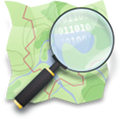
\includegraphics[width=0.5\textwidth]{../../img/osm.png}
				\vspace{1cm}
				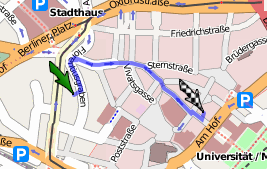
\includegraphics[width=0.8\textwidth]{../../img/openrouteservice.png}
			\end{center}
		\end{column}
	\end{columns}
\end{frame}

\note{Auch bei Kartendiensten gibt es eine gute Alternative zu Google Maps. Das OpenStreetMap Projekt funktioniert ein bisschen wie die Wikipedia, jeder kann Häuser kartographieren oder Informationen wie die Öffnungszeiten von Läden. Die Informationen sind meist sehr detaillert, in vielen Gegenden ist Mülleimern bis Wanderwegen alles eingetragen. Insbesondere in der Natur (Wander- und Mountainbikewege) oder auf Reisen (z.B. Indien) sind die Karten von OpenStreetmap deutlich besser. Gute mobile Apps die die Daten nutzen sind: OsmAnd (Android) und Maps.me (iOS).}
